\newcommand{\matl}{\mbox{\sc Matlab}}

\sect{Introduction to Matlab}

\ssect{Introduction}

{\bf What is \matl\ ?}
\begin{itemize}
 \item \matl\ (abbr. for MATrix LABoratory) is a software package for
numerical computation and visualization. The main part consists of a huge number
of build-in functions (e.g. linear Algebra, solving differential equations).
 \item \matl\ is primarily a numerical computation package, while {\sc Mathematica} and
{\sc Maple} are primarily symbolic algebra packages.
 \item Major \matl\ ``clones'': {\sc Scilab}, {\sc Octave}

\end{itemize}

{\bf Basic features:}
\begin{itemize}
 \item Automatic dimensioning (i.e., no dimension statements are required for
vectors or arrays,
 \item Case sensitivity (e.g., \verb(a( and \verb(A( are different variables)
 \item Build-in function are based on and optimized for vector and matrix operations.
 \item File types:
   \begin{itemize}
    \item M-files: standard ASCII text files, with a \verb(.m( extension,
    \item Mat-files: binary data files, with a \verb(.mat( extension,
    \item Mex-files: \matl{}-callable Fortran of C programs, with a \verb(.mex( extension,
   \end{itemize}
 \item The fundamental data type is the array which encompasses
several distinct data objects: integers, doubles, matrices, character
strings, structures, and cells.
 \item Data objects do not need to be declared as specific data types,
e.g.,there is no need to declare variables as real or complex.
\end{itemize}



\clearpage

\ssect{Basics}

\sssect{Graphical User Interface of \matl}

$\phantom{x}$


\begin{Figure}[ht]
  \centering
  \psfrag{1}[][]{\parbox{6cm}{\footnotesize{\sl Command Window:}\\ 
                 Entering of commands and data.\\ Results are displayed here.}}
  \psfrag{2}[][]{\parbox{5cm}{\footnotesize{\sl Workspace:}\\ 
                 List of used variables.}}
  \psfrag{3}[][]{\parbox{5cm}{\footnotesize{\sl Command History:}\\
                 List of used commands.}}
  \psfrag{4}[][t]{\parbox{10cm}{\footnotesize{\sl Working Path:}
                 Directory of source (e.g. m-files.)}}
  \psfrag{5}[b][b]{\parbox{4.6cm}{\footnotesize{\sl Tab of Current Dircetory:}\\
                 Browsing in the working path.}}
  \includegraphics[width=0.9\textwidth]{sec5_matlab/matlab_gui.eps}
  \caption{Components of \matl\ 's GUI} 
\end{Figure}

\clearpage

\sssect{Additional Environments}
$\phantom{x}$

\begin{Figure}[h]
  \centering
  \psfrag{1}[tl][tl]{\parbox{6cm}{\footnotesize\color{red}Run actual script}}
  \psfrag{2}[l][l]{\parbox{3cm}{\footnotesize \leftline{Tabbing between} \leftline{different scripts}}}
  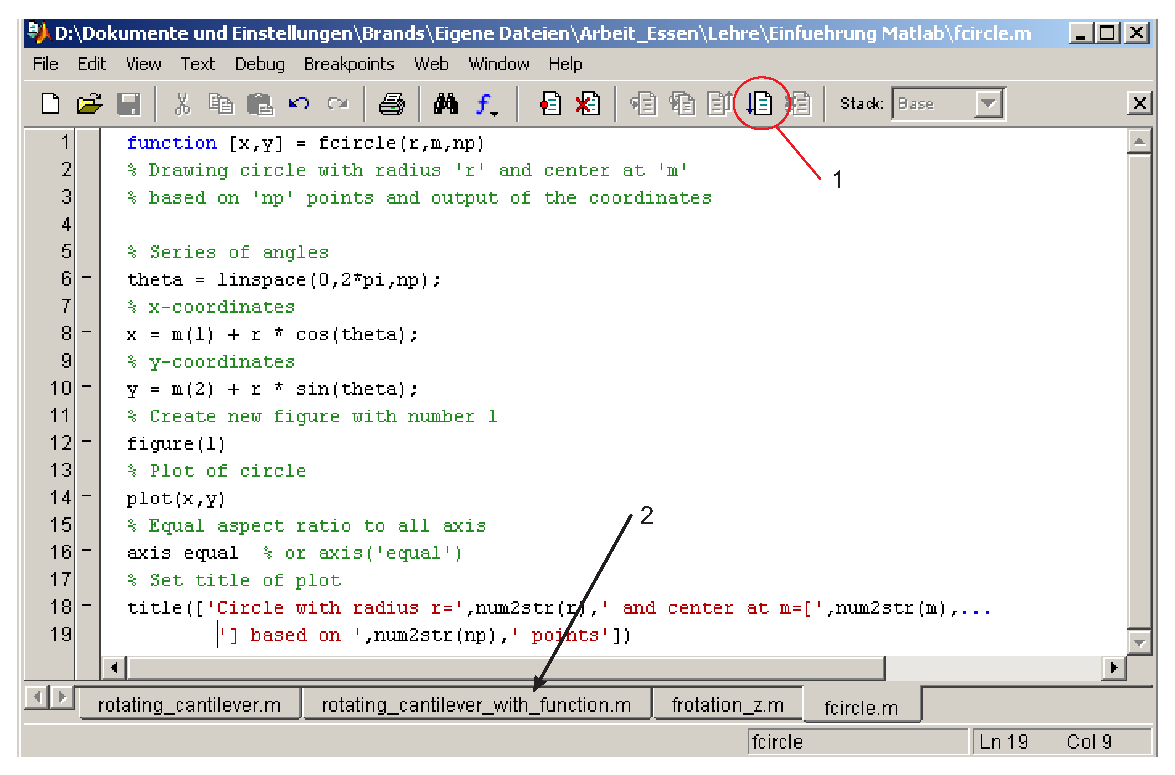
\includegraphics[width=0.85\textwidth]{sec5_matlab/matlab_editor.eps}
  \caption{M-Editor} 
\end{Figure}

\begin{Figure}[h]
  \centering
  \psfrag{1}[l][l]{\parbox{6cm}{\footnotesize\color{red} Zooming tools}}
  \psfrag{2}[l][l]{\parbox{5cm}{\footnotesize\color{red} Rotating tool}}
  \psfrag{3}[l][l]{\parbox{6cm}{\footnotesize\color{red} Insert objects}}
  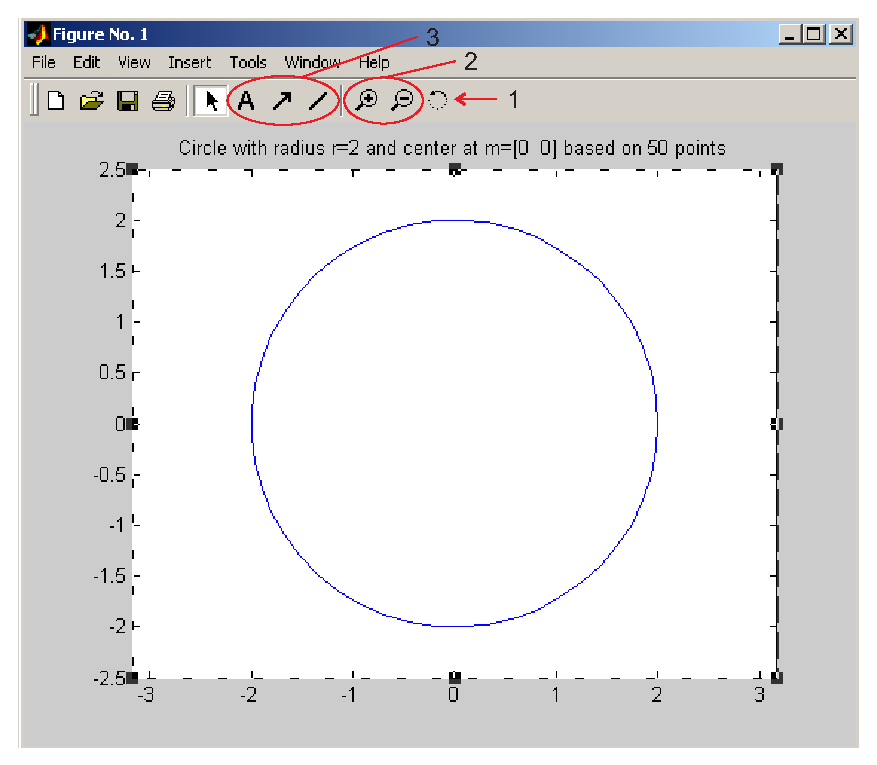
\includegraphics[width=0.65\textwidth]{sec5_matlab/matlab_fig.eps}
  \caption{Figure window} 
\end{Figure}

\clearpage
\sssect{General Commands}
$\phantom{x}$

\begin{tabular}{ll}
\multicolumn{2}{c}{\bf Help}\\
\multicolumn{2}{c}{\rule{0.97\textwidth}{0pt}}\\[-2ex]\hline
\verb(help <command>( & help on \verb(<command>(\\
\verb(lookfor <string>( & lists help containing \verb(<string>(\\
\hline
\end{tabular}

\begin{tabular}{ll}
\multicolumn{2}{c}{\bf Directory Operations}\\
\multicolumn{2}{c}{\rule{0.97\textwidth}{0pt}}\\[-2ex]\hline
\verb(pwd( & show current directory\\
\verb(cd( & change directory\\
\verb(dir( / \verb(ls( & list contents of current directory\\
\hline
\end{tabular}\\

%\vspace*{0.5cm}
\underline{Example:}\\[-5ex]
{\small\begin{verbatim}
>> help cos
 COS    Cosine.
    COS(X) is the cosine of the elements of X. 
 Overloaded methods
    help sym/cos.m
\end{verbatim}}

\sssect{Variables}
$\phantom{x}$

\begin{tabular}{ll}
\multicolumn{2}{c}{\bf Operators}\\
\multicolumn{2}{c}{\rule{0.97\textwidth}{0pt}}\\[-2ex]\hline
\verb(=( & assignment of value\\
\verb(+ - * / ^( & mathematical operators\\
\verb(,( (at end of line) & command with ouput\\
\verb(;( (at end of line) & no output\\
\verb(...( & linebreak inside of a command\\
\hline
\end{tabular}

\begin{tabular}{ll}
\multicolumn{2}{c}{\bf Fix Values}\\
\multicolumn{2}{c}{\rule{0.97\textwidth}{0pt}}\\[-2ex]\hline
\verb(i,j( & imaginary value $\sqrt{-1}$\\
\verb(pi( & $\pi = 3.14\ldots$\\
\verb(inf(  & infinity $\inf$\\
\verb(NaN(  & Not a Number, e.\ g.\ $\frac{0}{0}$\\
\verb(eps( & smallest displayable positive number\\
\hline
\end{tabular}

\begin{tabular}{ll}
\multicolumn{2}{c}{\bf Management of Variables}\\
\multicolumn{2}{c}{\rule{0.97\textwidth}{0pt}}\\[-2ex]\hline
\verb(who( & lists variables currently in workspace by name\\
\verb(whos( & lists variables with their size\\
\verb(clear( & clear workspace\\
\verb(clear <var>( & clear variable <var>\\
\verb(clc( / \verb(clf( / \verb(cla( & clear command / figure / axes\\
\hline
\end{tabular}\\
More information: type \verb/help +/ at \matl\ -commandline.

\underline{Examples:}\\
\begin{minipage}[t]{0.5\textwidth}
\small\begin{verbatim}
>> ( 47 + 1e+02 * 1.5 + 4^2 ) / 4
ans =
   53.2500
\end{verbatim}
\end{minipage}
\hfill
\begin{minipage}[t]{0.49\textwidth}
\verb(ans( is the variable of the result of the last execution.
\end{minipage}\\

\begin{minipage}[t]{0.5\textwidth}
{\small\begin{verbatim}
>> a = ( 47 + 1e+02 * 1.5 + 4^2 ) / 4
a =
   53.2500
\end{verbatim}}
\end{minipage}
\hfill
\begin{minipage}[t]{0.49\textwidth}
The result is stored in variable \verb(a(. execution.
\end{minipage}\\

\sssect{Mathematical Functions}\vspace*{-0.2cm}
$\phantom{x}$

\begin{tabular}{ll}
\multicolumn{2}{c}{\rule{0.97\textwidth}{0pt}}\\[-2ex]\hline
\verb/sqrt(x)/ & square root\\
\verb/xp(x)/ & exponential funktion\\
\verb/log(x)/ / \verb/log10/ & logarithms\\
\verb/sin(x)/ & sinus\\
\verb/cos(x)/ & cosin\\
\verb/tan(x)/ & tangens\\
\verb/atan(x)/ & arcus-tanges (angle $-90^{\circ}\ldots+90^{\circ}$)\\
\verb/atan2(y,x)/ & arcus-tanges (angle $-180^{\circ}\ldots+180^{\circ}$)\\
\verb/abs(x)/ & absolute value of \verb/x/\\
\verb/sign(x)/ & signum (sign of \verb/x/)\\
\hline
\end{tabular}\\
More information: type \verb/help elfun/ or
\verb/help datafun/ at \matl\ -commandline.


\underline{Example:}\\
\begin{minipage}[t]{0.5\textwidth}
\small\begin{verbatim}
>> y1 = 2^2+log(pi)*sin(0.75*pi/2)+sqrt(exp(2*pi/3))
y1 =
    7.9072
\end{verbatim}
\end{minipage}
\hfill
\begin{minipage}[t]{0.49\textwidth}
$$ y_1 = 2^2 + \ln \pi \sin(0.75\pi/2) + \sqrt{e^{2/3\pi}}$$
\end{minipage}

\sssect{Vectors and Matrices}\vspace*{-0.2cm}
$\phantom{x}$

\begin{tabular}{ll}
\multicolumn{2}{c}{\bf Formulation of vectors and matrices}\\
\multicolumn{2}{c}{\rule{0.97\textwidth}{0pt}}\\[-2ex]\hline
\verb/[ x1 x2 ...; y1,y2,...] / & vector or matrix ('\verb/,/' or space between\\
 &  columns, '\verb/;/' or linebreak between rows)\\
\verb/start:/ <\verb/stepsize:/> \verb/end/ & colon-operator (stepsize is opt., otherwise = 1)\\
\verb/linspace(start,end,num_steps)/ & linear row-vector\\
\verb/logspace(start,end,num_steps)/ & logarithmical row-vector\\
\verb/eye(rows,columns)/ & Identity [rows x cols]\\
\verb/ones(rows,columns)/ & matrix with all Elements equal 1 [rows x cols]\\
\verb/zeros(rows,columns)/ & zero-matrix [rows x cols]\\
\verb/rand(rows,columns)/ & random matrix [rows x cols]\\
\verb/a(index)/ & element of vector at position \verb/index/\\
\verb/A(r,c)/ & element of matrix at row \verb/r/ and column \verb/c/\\
\hline
\end{tabular}

\underline{Examples:}\\
\begin{minipage}[t]{0.5\textwidth}
\small\begin{verbatim}
>> x=[1 2 3]
x =
     1     2     3
>> y=[4;5;6]
y =
     4
     5
     6
>> A=[1 2 3;4,5,6;7 8,9]
A =
     1     2     3
     4     5     6
     7     8     9
>> A(2,3)
ans =
     6
\end{verbatim}
\end{minipage}
\hfill
\begin{minipage}[t]{0.5\textwidth}
\small\begin{verbatim}
>> A(1,2)=8
A =
     1     8     3
     4     5     6
     7     8     9
>> B=A(2:3,1:3)
B =
     4     5     6
     7     8     9
>> v=0:2:8
v =
     0     2     4     6     8
>> v=[8:-2:0]
v =
     8     6     4     2     0
\end{verbatim}
\end{minipage}

\sssect{Operations on Vectors and Matrices}
$\phantom{x}$

\begin{tabular}{ll}
\multicolumn{2}{c}{\bf Operations}\\
\multicolumn{2}{c}{\rule{0.97\textwidth}{0pt}}\\[-2ex]\hline
\verb(.* .\ ./ .^( & element-wise calculations\\
\verb(\ /( & left and right division\\
\verb/transpose(A)/ or \verb/A.'/ & transpose of \verb/A/\\
\verb/ctranspose(A)/ or \verb/A'/ & transpose of \verb/A/ (conjugated complex)\\
\verb/inv(A)/ & inverse of \verb/A/\\
\verb/det(A)/ & determinant of \verb/A/\\
\hline
\end{tabular}

\begin{tabular}{ll}
\multicolumn{2}{c}{\bf Dimensions}\\
\multicolumn{2}{c}{\rule{0.97\textwidth}{0pt}}\\[-2ex]\hline
\verb/[M,N] = SIZE(A)/ & dimension of matrix and vector\\
\verb/M = SIZE(A,DIM)/ & length of matrix of dimension \verb/DIM/\\
\hline
\end{tabular}

\begin{tabular}{ll}
\multicolumn{2}{c}{\bf Mathematical Functions for Vectors and Matrices}\\
\multicolumn{2}{c}{\rule{0.97\textwidth}{0pt}}\\[-2ex]\hline
\verb/sum(a)/ & sum of vector elements\\
\verb/prod(a)/ & product of vector elements\\
\verb/min(a)/ & smallest vector element\\
\verb/max(a)/ & largest vector element\\
\verb/sort(a)/ & element in increasing order\\
\verb/find(a)/ & non-zero elements\\
\hline
\end{tabular}

\medskip
\underline{Examples:}\\
\begin{minipage}[t]{0.5\textwidth}
\small\begin{verbatim}
>> A=[1 2 3; 4 5 6; 7 8 9];
>> B=[1 2 3; 2 4 5; 3 7 8];
>> b=[2 4 6 8 10]';
>> v=0:2:8;

>> v*b
ans =
   160
>> v'*b'
ans =
     0     0     0     0     0
     4     8    12    16    20
     8    16    24    32    40
    12    24    36    48    60
    16    32    48    64    80
\end{verbatim}
\end{minipage}
\hfill
\begin{minipage}[t]{0.5\textwidth}
\small\begin{verbatim}
>> c=v+b';
>> c=v-b';
>> C=A+B;
>> C=A-B;
>> C=A*B;
>> c=A*v(1:3)'
c =
    16
    34
    52
>> c=v.*b'
c =
     0     8    24    48    80
\end{verbatim}
\end{minipage}

\medskip
\underline{Example:}\\
\begin{minipage}[t]{0.4\textwidth}
\small\begin{verbatim}
>> A=[5 -3 2; -3 8 4; 2 4 -9];
>> b=[10;20;9];
>> x=A\b
x =
    3.4442
    3.1982
    1.1868
\end{verbatim}
\end{minipage}
\hfill
\begin{minipage}[t]{0.59\textwidth}
Solving the linear system of equations: $\bA\bx = \bb$
\begin{eqnarray*}
5x &=& 3y-2z+10\\
8y+4z &=& 3x+20\\
2x+4y-9z &=& 9\\
\end{eqnarray*}
\end{minipage}

\clearpage
\sssect{Scripts and Functions}
$\phantom{x}$

\begin{itemize}
\item Script:\\
  When you invoke a script, MATLAB simply executes the commands found in the file. Scripts can operate on existing data in the workspace, or they can create new data on which to operate. Although scripts do not return output arguments, any variables that they create remain in the workspace, to be used in subsequent computations. 
\item Function:\\
  Functions are \verb/.m/-files that can accept input arguments and return output arguments. The name of the \verb/.m/-file and of the function should be the same. Functions operate on variables within their own workspace, separate from the workspace you access at the MATLAB command prompt.
\end{itemize}
Both types of codes are stored as .m-file.

\underline{Structure of functions:}
{\small\begin{verbatim}
function [a_out,b_out] = name_of_function(a_in,b_in)
%         output list                     input list
%
% Description of function can be placed here
% by using the comment-operator '%'. This
% informations can be displyed by typing
% 'help name_of_function' at MATLAB-command-line.
.
.
a_out = a_in - a_out;
b_out = a_in + a_out;
.
.
\end{verbatim}}

\underline{Example: Computation of the length of a vector}
{\small\begin{verbatim}
function vlength = fvectorlength(vector)
%
% Computation of the length 'vlength' of
% a column vector 'vector'

vlength = sqrt(vector'*vector);
\end{verbatim}}
Calling the function:
{\small\begin{verbatim}
>> fvectorlength([-1;3;5])
ans =
    5.9161
\end{verbatim}}

\clearpage
\sssect{Relational and Logical Operators}\vspace*{-0.2cm}
$\phantom{x}$

\begin{tabular}{llll}
\multicolumn{4}{c}{\rule{0.97\textwidth}{0pt}}\\[-2ex]\hline
\verb(== , ~=( & equal, not equal\\
\verb(< , <=( & less than, less than or equal\\
\verb(> , >=( & greater than, greater than or equal\\
\hline
\verb/~/ & logical not & \verb/&/ & element-wise logical AND\\
\verb/|/ & element-wise logical OR & \verb/xor/ & logical EXCLUSIVE OR\\
\hline
\end{tabular}\\
More informations: type \verb/help +/ at \matl\ -commandline.

\sssect{IF-/CASE Statements and Loops}\vspace*{-0.2cm}
$\phantom{x}$

\begin{tabular}{ll}\hline
\verb(IF( expression (e.g. \verb/a==1/)& IF statement condition\\
  \hspace*{0.3cm} statements\\
\verb(ELSEIF( expression & The ELSE and ELSEIF parts\\
  \hspace*{0.3cm} statements &  (optional)\\
\verb(ELSE(\\
  \hspace*{0.3cm} statements\\
\verb(END(\\
\hline
\verb(SWITCH( switch-expr (e.g. \verb/id/)& SWITCH statement case \\
\verb(  CASE( case-expr, (e.g. \verb/1/) \\
  \hspace*{0.6cm} statement, ..., statement\\
\verb(  CASE {(case-expr1, case-expr2, case-expr3,...\verb(}(\\
  \hspace*{0.6cm} statement, ..., statement\\
\verb(  OTHERWISE,(\\
  \hspace*{0.6cm} statement, ..., statement\\
\verb(END(\\
\hline
\verb(FOR( variable = expr (e.g. \verb/ii=1:10/)& Repeat statements a specific\\
  \hspace*{0.3cm} statement, ..., statement & number of times.\\
\verb(END(\\
\hline
\verb(WHILE( expression (e.g. \verb/ii<imax/)& Repeat statements an \\
  \hspace*{0.3cm} statements & indefinite number of times.\\
\verb(END(\\
\hline
\end{tabular}

\sssect{Plotting Figures}\vspace*{-0.2cm}
$\phantom{x}$

\begin{tabular}{ll}
\multicolumn{2}{c}{\bf Control the figure window}\\
\multicolumn{2}{c}{\rule{0.97\textwidth}{0pt}}\\[-2ex]\hline
\verb/figure , figure(no)/ & create, activate figure with number \verb/no/\\
\verb/subplot(num_rows,num_cols,index)/ & create a subplot\\
& e.g., \verb/subplot(2,3,2)/: subplot with 2 rows\\
& and 3 column, activate 2$^{nd}$ subplot\\
\verb/gcf/ & handle of active figure\\
\verb/clf/ & clear active figure\\
\verb/delete(id)/ & delete object with handle \verb(id(\\
\verb/close(index)/ & delete figure window \verb(index(\\
\verb/close all /& delete all figure windows\\
\verb/hold/ <\verb/on/ | \verb/off/> & keeping existent objects through\\
& new plots on/off \\
\hline
\end{tabular}

\begin{tabular}{ll}
\multicolumn{2}{c}{\bf 2-D Plot Commands}\\
\multicolumn{2}{c}{\rule{0.97\textwidth}{0pt}}\\[-2ex]\hline
\verb/plot(/ <\verb/x,/> \verb/y/ <\verb/,plotstyle/> \verb/,...)/& plot, linear (<> = opt.)\\
\verb/fplot(func,range)/ & plot of explicit function\\
\verb/line(x,y)/ & Create line through coordinate-vectors \verb/x,y/\\
\verb/text(x,y,string)/ & Place text \verb/string/ at position \verb/x,y/\\
\multicolumn{2}{l}{For more informations about 2-D Plots, call {\ttfamily help plot} at command-line.}\\
\hline
\end{tabular}

\begin{tabular}{ll}
\multicolumn{2}{c}{\bf 3-D Plot Commands}\\
\multicolumn{2}{c}{\rule{0.97\textwidth}{0pt}}\\[-2ex]\hline
\verb/plot3(x,y,z /<\verb/,plotstyle/> \verb/,...)/ & threedimensional plot\\
\verb/sphere/ & plot a sphere\\
\verb/[x,y,z] = sphere/ & store coordinates of a unit sphere to \verb/x,y,z/\\
\verb/line(x,y,z)/ & Create line through coordinate-vectors \verb/x,y,z/\\
\verb/text(x,y,z,string)/ & Place text \verb/string/ at position \verb/x,y,z/\\
\hline
\end{tabular}

\begin{tabular}{lll|lll}
\multicolumn{6}{c}{\bf Plotstyles}\\
\multicolumn{6}{c}{\rule{0.97\textwidth}{0pt}}\\[-2ex]\hline
\multicolumn{3}{c}{colors:} & \multicolumn{3}{c}{lines and markes:}\\
\verb/k/ black & \verb/r/ red & \verb/g/ green & 
\verb/-/ solid    & \verb\o\ circle & \verb/./ points\\
\verb/b/ blue  & \verb/m/ magenta & \verb/w/ white &
\verb/--/ dashed  & \verb\*\ star & \verb\x\ x-mark\\
\verb/c/ cyan  & \verb/y/ yellow & &
\verb/:/ dotted   & \verb\+\ plus & \verb/-./ dashdot\\
More infos: \verb/help plot/\\
\hline
\end{tabular}\\[2ex]

\begin{minipage}[c]{0.54\textwidth}
\underline{Examples:}
\small\begin{verbatim}
>> figure(1)
>> clf
>> t=0:pi/20:2*pi;
>> plot(t,sin(t),'-.r*')
>> hold on
>> plot(t,(sin(t-pi/2)),'linestyle','--',...
   'marker','o','color','m')
>> plot(t,sin(t-pi),':bs')
>> hold off
\end{verbatim}
\end{minipage}
\hfill
\begin{minipage}[c]{0.45\textwidth}
\centering
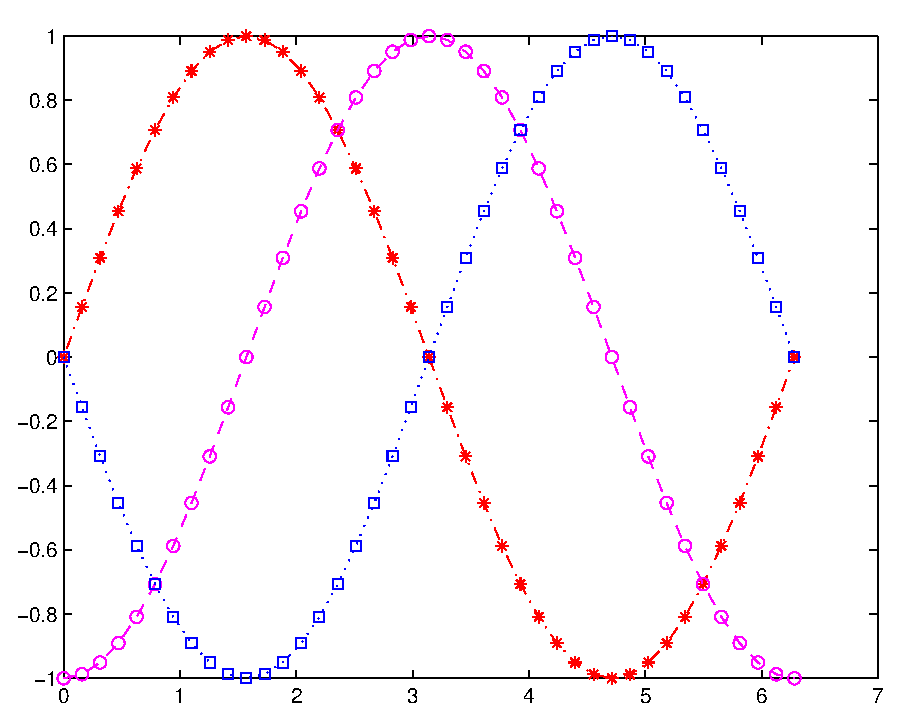
\includegraphics[width=0.8\textwidth]{sec5_matlab/plot_example.eps}
\end{minipage}\\[1cm]

\begin{tabular}{ll}
\multicolumn{2}{c}{\bf Labelling of Axes and Figures}\\
\multicolumn{2}{c}{\rule{0.97\textwidth}{0pt}}\\[-2ex]\hline
\verb/axis([xmin,xmax,ymin,ymax/ <\verb/,zmin,zmax/> \verb/])/ & scaling (min=\verb/-inf/ or\\
& max=\verb/inf/ $\rightarrow$ auto scal.) \\
\verb/axis/ <\verb/on | off | auto | equal | square/> & several axis commands\\
& more: \verb/help axis/\\
\verb/grid/ <\verb/on | off/> & grid\\
\verb/gca/ & handle to current axis\\
\verb/cla/ & delete current axis\\
\verb/xlabel(string)/ & label of x-axis\\
\verb/ylabel(string)/ & label of y-axis\\
\verb/zlabel(string)/ & label of z-axis\\
\verb/title(string)/ & title of current axis\\
\verb/legend(string_1,string_2,.../ <\verb/,pos/> & place legend\\
& \verb/pos = 0,1,2,3,4,-1/\\
\hline
\end{tabular}
 

\ssect{Exercises}

\sssect{\label{sec:exp1}Animation of a rotating cantilever}
$\phantom{x}$

\begin{minipage}[t]{0.5\textwidth}
The cantilever with the length~$L$ is fixed at the top (point P2)
of a vertical rod (height~$H$).
Both include an angle~$\alpha$. The vertical rod is bounded
by a revolute joint at its base (point P1) with the $z$-axis as rotation axis. At the free end of the
cantilever (point P3) a ball is attached and its radius is~$R$.\smallskip\\
Program a \matl -script (\verb/.m/-file), which animates the rotation of
the beside shown system about
the vertical axis ($z$-axis) with angle~$\varphi$.
\end{minipage}
\hfill
\begin{minipage}[t]{0.39\textwidth}
\begin{picture}(0,0)
\unitlength1cm
\put(0.0,-5.0){\scalebox{0.8}{\input{sec5_matlab/bild1020.pstex_t}}}
\end{picture}
\end{minipage}


\sssect{\label{sec:exp2}Animation of a rotating cantilever using a subroutine}
$\phantom{x}$

The \matl -script in Section \ref{sec:exp1} should be modified.
Now a self-programed function should compute the rotated coordinates
for the animation. The input-parameters should be the
original coordinates and the rotation angle~$\varphi$. The output of the
function should be the rotated coordinates.

\clearpage
\sssect{Source code}
$\phantom{x}$

{\bf to Section~\ref{sec:exp1}}\\[-6ex]
\begin{alltt}
\small
\input{sec5_matlab/rotating_cantilever.m}
\end{alltt}

\vspace*{-0.5cm}
{\bf to Section~\ref{sec:exp2}}\smallskip\\
Replaced parts in the \matl -script:
\vspace*{-1cm}
\begin{alltt}
\small
...
\input{sec5_matlab/rotating_cantilever_with_function_(new_parts).m}
...
\end{alltt}


\vspace*{-0.1cm}
New function \verb/frotation/:
\vspace*{-0.9cm}
\begin{alltt}
\small
\input{sec5_matlab/frotation_z.m}
\end{alltt}
